%%
% La siguiente plantilla esta basada en el siguiente enlace:
% http://academic.reed.edu/physics/courses/Physics332.s08/reports.html
% La plantilla original puede descargarse de ese sitio
% Se dejo parte del texto original en inglés para ilustar el uso de la plantilla
% Se hicieron algunas modificaciones para ajustar el idioma y otros detalles para 
% completar un reporte técnico breve pero muy puntual
% Modificación Inicial: Marco Aurelio Nuno Maganda - 11/SEP/2014
% 
% Enlace a la documentación del tipo de documento base (revtex4)
% http://mirror.hmc.edu/ctan/macros/latex/contrib/revtex/doc/latex/revtex/source/revtex4-1.pdf
%
% En algunas distribuciones es necesario instalar el paquete texlive-publishers
%
%\documentclass[letterpaper,aps,twocolumn,pre,nofootinbib]{revtex4}
%\documentclass[twocolumn]{article}
\documentclass[conference]{IEEEtran}

\usepackage[spanish]{babel}
\usepackage{amsmath,amssymb,amsfonts,amsthm}
\usepackage{graphicx}
%\usepackage{bbm}
\usepackage[utf8]{inputenc} % Caracteres en Español (Acentos, ñs)
\usepackage{url} % ACENTOS
\usepackage{hyperref} % Referencias
\usepackage{subfig}
\usepackage{lipsum}
\usepackage{balance}


%%%%%%%%%%%%%%%%%%%%%%%%%%%%%%%%%%%%%%%%%%%%%
% PARCHE PARA ELIMINAR LA FECHA DEL DOCUMENTO
% 
\usepackage{etoolbox}
\makeatletter
% \frontmatter@RRAP@format is responsible for the parentheses
\patchcmd{\frontmatter@RRAP@format}{(}{}{}{}
\patchcmd{\frontmatter@RRAP@format}{)}{}{}{}
%\renewcommand\Dated@name{}
\makeatother	
% FIN DEL PARCHE
% 
%%%%%%%%%%%%%%%%%%%%%%%%%%%%%%%%%%%%%%%%%%%%%

%%%%%%%%%%%%%%%%%%%%%%%%%%%%%%%%%%%%%%%%%%%%%
% PARCHE PARA PERMIRIR UTILIZAR BIBLATEX EN ESTA PANTLLA
%\PassOptionsToPackage{square,numbers}{natbib}
%\RequirePackage{natbib}  
%%%%%%%%%%%%%%%%%%%%%%%%%%%%%%%%%%%%%%%%%%%%%

\usepackage[backend=bibtex,sorting=none]{biblatex}
% Estas lineas permiten romper los hipervinculos muy largos !!!!
\setcounter{biburllcpenalty}{7000}
\setcounter{biburlucpenalty}{8000}
\addbibresource{references.bib}

% Actualiza en automático la fecha de las citas de internet a la fecha de la compilación del documento
\usepackage{datetime}
\newdateformat{specialdate}{\twodigit{\THEDAY}-\twodigit{\THEMONTH}-\THEYEAR}
\date{\specialdate\today}

% la sentencia \burl en las citas... 
\usepackage[hyphenbreaks]{breakurl}

\renewcommand\spanishtablename{Tabla}
\renewcommand\spanishfigurename{Figura}

%\usepackage{datetime}
%\newdateformat{specialdate}{\twodigit{\THEDAY}-\twodigit{\THEMONTH}-\THEYEAR}
%\newdateformat{specialdate}{\twodigit{\THEDAY}-\THEYEAR}
%\date{\specialdate\today}


\begin{document}
%%%%%%%%%%%%%%%%%%%%%%%%%%%%%%%%%%%%%%%%%%%%%
% Definitions
%
%
% Define your special symbols here
%
%%%%%%%%%%%%%%%%%%%%%%%%%%%%%%%%%%%%%%%%%%%%%

% use to set width of figures
\newcommand{\breite}{1.0} %  for twocolumn
\newcommand{\RelacionFiguradoscolumnas}{0.9}
\newcommand{\RelacionFiguradoscolumnasPuntoCinco}{0.45}


%%%%%%%%%%%%%%%%%%%%%%%%%%%%%%%%%%%%%%%%%%%%%
% End Definitions
%%%%%%%%%%%%%%%%%%%%%%%%%%%%%%%%%%%%%%%%%%%%%


%Title of paper
\title{Demo de Realidad Virtual de la UPV: Integración del Edificio C, Cafetería Grande y Pequeña}


% En caso de trabajos en equipo, poner a todos los autores en estricto ORDEN ALFABETICO
\author{\IEEEauthorblockN{Carlos Emiliano Cortes Moctezuma\IEEEauthorrefmark{1}, 
	César Alfonso Montes López\IEEEauthorrefmark{1},
	Jorge Alberto Rios Mendoza\IEEEauthorrefmark{1},\\
	Grecia Yarezy Rodriguez Dominguez\IEEEauthorrefmark{1},
	Jennifer Elizabeth Yepez Lopez\IEEEauthorrefmark{1}}
		
\IEEEauthorblockA{\IEEEauthorrefmark{1}Ingeniería en Tecnologías de la Información\\
Universidad Politécnica de Victoria}
}

%\date{}

\maketitle

\begin{abstract} 
\textbf En el presente informe se describe el desarrollo de una aplicación móvil de Realidad Virtual diseñada para la exploración de las instalaciones de la Universidad Politécnica de Victoria. Fue desarrollada en Android Studio utilizando Java y OpenGL ES, destacando el uso de GLSurfaceView para el renderizado de gráficos en tiempo real. El sistema permite al usuario interactuar con un entorno virtual que integra nuevos edificios: la Cafetería Grande, la Cafetería Pequeña y el Edificio C, los cuales cuentan con texturas personalizadas, interiores y escaleras. La navegación se realiza combinando el uso de un control externo para el desplazamiento y los sensores de movimiento del dispositivo para orientar la vista de forma natural. Adicionalmente, la aplicación integra un minimapa dinámico que se actualiza según la ubicación del usuario, facilitando la orientación espacial dentro del universo virtual.
\end{abstract}


%\maketitle must follow title, authors, abstract, \pacs, and \keywords


\section{Introducción}

La visualización de espacios arquitectónicos ha evolucionado significativamente gracias a la Realidad Virtual (RV), permitiendo que los usuarios exploren espacios universitarios de forma inmersiva desde sus dispositivos móviles. Con el uso de OpenGL ES en el sistema operativo Android, es posible construir entornos tridimensionales donde el usuario percibe profundidad y escala de manera realista, facilitando la comprensión de la distribución espacial de una institución \cite{Chin2012}. Esta aplicación expande el demo original de la universidad mediante la integración de nuevas estructuras detalladas: el Edificio C, la Cafetería Grande y la Cafetería Pequeña, ofreciendo una representación más completa y funcional del entorno institucional.

Para que la exploración sea intuitiva, el sistema permite que el usuario se desplace entre los edificios mediante un control externo, mientras que la orientación de la vista se ajusta en tiempo real al mover el dispositivo. El diseño del entorno se enfoca en que el usuario pueda no solo observar las fachadas, sino también entrar a los edificios para visualizar detalles como escaleras y mobiliario, logrando una transición fluida entre el exterior y el interior. Esto se consigue mediante el cálculo de vectores de cámara que definen con precisión la posición y la dirección de la mirada dentro del universo virtual \cite{LearnOpenGLCamera2026}.

El funcionamiento de esta herramienta se apoya directamente en el hardware del teléfono móvil para garantizar una experiencia fluida. Al capturar la rotación del dispositivo mediante sensores especializados, la aplicación sincroniza los movimientos físicos del usuario con la cámara virtual, asegurando que la navegación sea natural \cite{AndroidSensors2026}.

\section{Desarrollo Experimental}

Como primer paso para la expansión del universo virtual, se procedió a la definición de la nueva geometría tridimensional dentro de la clase CubeRenderer.java. Para la creación de la Cafetería Grande, la Cafetería Pequeña y el Edificio C, se programaron algoritmos que calculan arreglos de vértices para formar prismas rectangulares y cuadrangulares sólidos. Estas estructuras se renderizan mediante glDrawArrays, que permite que la GPU procese los puntos en el espacio para construir las paredes y techos que delimitan cada edificio \cite{KhronosDrawArrays2026}.

\vspace{0.2cm}

El siguiente avance consistió en la aplicación de realismo visual mediante el mapeo de texturas 2D. Se integraron recursos en formato .png para diferenciar las fachadas de los interiores; por ejemplo, para la Cafetería Grande se cargaron imágenes específicas para el frente exterior y los lados internos. Este proceso se apoya en la función glTexImage2D, que transfiere los datos de los píxeles de las imágenes almacenadas en la carpeta res/drawable hacia la memoria de video, permitiendo que cada muro base de color blanco adquiera la apariencia detallada de una estructura real con puertas y letreros \cite{KhronosTexImage2026}.

\vspace{0.2cm}

Posteriormente, se trabajó en el diseño arquitectónico interno y la inmersión. Para permitir que el usuario entre a los edificios, se duplicó la geometría de las paredes apuntando hacia el interior y se separaron ligeramente de las paredes exteriores. Este ajuste técnico es fundamental para evitar el fenómeno de Z-fighting o parpadeo de texturas, asegurando que al estar dentro del cubo se visualice una superficie sólida y blanca \cite{Akenine2018}. Dentro de estos espacios se añadieron elementos de mobiliario como mesas de madera y sillas negras, construidos mediante bloques geométricos escalados para simular un ambiente funcional.

\vspace{0.2cm}

El siguiente paso en el desarrollo de la aplicación, fue la implementación de las escaleras para permitir el acceso a los niveles superiores. Para el Edificio C y la Cafetería Grande, se diseñaron escaleras rectas utilizando bucles que generan una sucesión de prismas pequeños desplazados en los ejes Y y Z. En la Cafetería Grande, las escaleras se colocaron pegadas a la pared del fondo, con un diseño angosto y descendente que permite subir al techo sin obstruir la visibilidad del área de mesas. Este método de dibujo paramétrico facilita que los objetos complejos se integren de manera simétrica en el entorno virtual \cite{AndroidGraphics2026}.

\vspace{0.7cm}

La siguiente actividad se centró en la configuración de la navegación mediante el control físico y los sensores. En la Tabla \ref{Tab:Control} se detalla la configuración final de los botones del gamepad vinculados en la lógica de MainActivity.java para interactuar con el mundo de Realidad Virtual.

\begin{table}[h!]
	\centering
	\renewcommand{\arraystretch}{1.3}
	\caption{Mapeo de funciones del control físico.}
	\label{Tab:Control}
	\begin{tabular}{|l|l|}
		\hline
		\textbf{Botón del Control} & \textbf{Acción en la Aplicación} \\ \hline
		Arrow Button (Arriba)          & Desplazamiento hacia enfrente. \\ \hline
		Arrow Button (Abajo)          & Desplazamiento hacia atrás. \\ \hline
		Arrow Button (Izquierda)           & Desplazamiento a lado izquierdo. \\ \hline
		Arrow Button (Derecha)        & Desplazamiento a lado derecho. \\ \hline
		Botón Y                    & Inclinar la cámara hacia arriba. \\ \hline
		Botón A                    & Inclinar la cámara hacia abajo. \\ \hline
		Botón X                    & Cambiar de edificio. \\ \hline
		Botón B                    & Cerrar aplicación. \\ \hline
	\end{tabular}
\end{table}

\vspace{0.2cm}

Para que la exploración fuera natural, se realizó un ajuste en el procesamiento del sensor de vector de rotación. Se detectó que el eje vertical estaba invertido, por lo que se modificó el signo del componente en el método de actualización de la vista; esto permitió que al inclinar físicamente el celular hacia arriba, el usuario visualice el cielo y no el suelo. Además, se programó un cálculo matemático para determinar la dirección lateral exacta en función de hacia dónde está mirando el usuario en cada momento. Al combinar la dirección de la mirada con el eje vertical del mundo (el cielo), la aplicación identifica cuál es el lado derecho e izquierdo real del usuario. Esto garantiza que las direcciones del control coincidan con lo que el usuario ve en pantalla, evitando que en la app se mueva hacia el lado contrario \cite{Dunn2011}.

\vspace{0.2cm}

En cuanto a la orientación espacial, se programó un sistema de sincronización entre la navegación y el minimapa para que el usuario siempre sepa en qué parte de la universidad se encuentra. Cada vez que el usuario presiona el botón X del control para cambiar de edificio, la aplicación realiza dos acciones al mismo tiempo: primero, mueve la cámara automáticamente para que el usuario aparezca justo frente a la puerta del edificio elegido, y segundo, cambia la imagen del mapa que se muestra en la esquina de la pantalla. Esto significa que si el usuario viaja a la Cafetería Grande, el mapa se actualizará solo para mostrar esa área específica, evitando confusiones y permitiendo que la posición marcada en el minimapa coincida exactamente con lo que el usuario está viendo en el mundo de Realidad Virtual \cite{Silva2012}.

\vspace{0.2cm}

También, se optimizó el entorno global para soportar la expansión del mapa. Como los nuevos edificios se construyeron en zonas más alejadas del punto de inicio, fue necesario agrandar todo el escenario virtual para que el suelo y el cielo alcanzaran a cubrir esas nuevas áreas. Si no se hubiera hecho este ajuste, al viajar a la cafetería el usuario vería que el césped se termina de repente, dejando ver un vacío negro debajo y alrededor del edificio. Por ello, se amplió el tamaño del plano de césped y las dimensiones del cielo hasta las 6000 unidades. Esta mejora asegura que el usuario siempre esté rodeado de escenario, sin importar qué tanto camine o hacia dónde gire la cabeza, manteniendo un horizonte completo y realista que envuelve toda la universidad sin cortes visuales ni espacios vacíos \cite{Ginsburg2014}.

\vspace{0.2cm}

Finalmente, como parte de los cambios realizados para la actualización del proyecto se realizaron las siguientes mejoras: 

\vspace{0.1cm}

\begin{itemize}
	\item Conectividad de pasillos: Se trazaron los caminos para conectar a todos los edificios (A, B, C, H, Im la Cafetería Grande y la Cafetería Pequeña).
	
	\vspace{0.2cm}
	
	\item Incorporación de la rotonda: Se añadió la rotonda con una jardinera en el centro.
	
	\vspace{0.2cm}
	
	\item Distribución real de edificios: Se reorganizó la posición de cada edificio en el mundo virtual para que coincida de forma parecida con la ubicación real de las instalaciones de la universidad.
	
	\vspace{0.2cm}
	
	\item Estructura del Edificio C: Se completó la construcción del Edificio C y se añadió el tragaluz en el mundo virtual, replicando el diseño de las instalaciones reales de la universidad.
	
	\vspace{0.2cm}
	
	\item Optimización de texturas: Se corrigió el problema de visibilidad de las imágenes. Ahora las texturas se mantienen nítidas y visibles incluso cuando la cámara se aleja, sin desaparecer repentinamente.
	
	\vspace{0.2cm}
	
	\item Corrección en los sensores del celular: Se mejoró la lógica de navegación móvil. Anteriormente, al mover el teléfono la vista respondía de forma invertida o descontrolada; ahora el movimiento es mas natural y se desplaza exactamente hacia donde el usuario dirige el dispositivo.
\end{itemize}

\vspace{0.2cm}

Con el propósito de facilitar la navegación en esta nueva versión que se desarrolló, se presenta la siguiente guía de flujo:

\begin{enumerate} 
	\item Al iniciar, el usuario puede explorar los edificios originales o usar el botón X para saltar directamente a las nuevas áreas.
	
	\vspace{0.2cm}
	
	\item Al llegar a la Cafetería Grande, el usuario aparecerá justo enfrente de la fachada blanca con el detalle de entrada central. Puede usar las flechas del arrow button para entrar y ver las mesas.
	
	\vspace{0.2cm}
	
	\item Al cambiar a la Cafetería Pequeña, se observará un edificio compacto. El usuario puede entrar para notar el espacio reducido y las dos mesas interiores.
	
	\vspace{0.2cm}
	
	\item En el Edificio C, desde el exterior el usuario puede apreciar las ventanas y jardineras características de la estructura. En el interior, se integraron elementos como una jardinera, puertas simuladas en las paredes y un tragaluz en el techo, permitiendo comprobar además la fluidez del movimiento vertical mediante los sensores del dispositivo.
	
\end{enumerate}

\vspace{0.3cm}

\section{Resultados}

A continuación, se describen los resultados obtenidos en las pruebas de funcionamiento de la aplicación:

\vspace{0.2cm}

En la Figura \ref{fig_otros_detalles}(a) se presenta el estado inicial de la aplicación, donde el usuario aparece siempre posicionado frente al Edificio A cuando inicia la app para establecer un punto de referencia claro. Por otro lado, la Figura \ref{fig_otros_detalles}(b) ilustra cómo el sistema sincroniza la posición del usuario con el minimapa, cargando automáticamente la representación visual correspondiente a la zona actual para facilitar la orientación dentro del entorno; adicionalmente, se muestra la respuesta del sistema al inclinar el teléfono físicamente hacia arriba, logrando que la cámara virtual apunte correctamente al cielo, lo cual formó parte de las correcciones de navegabilidad implementadas para asegurar un movimiento fluido y natural.

\vspace{0.3cm}

\begin{figure}[h!]
	\centering
	\subfloat[Estado inicial (Edificio A).]{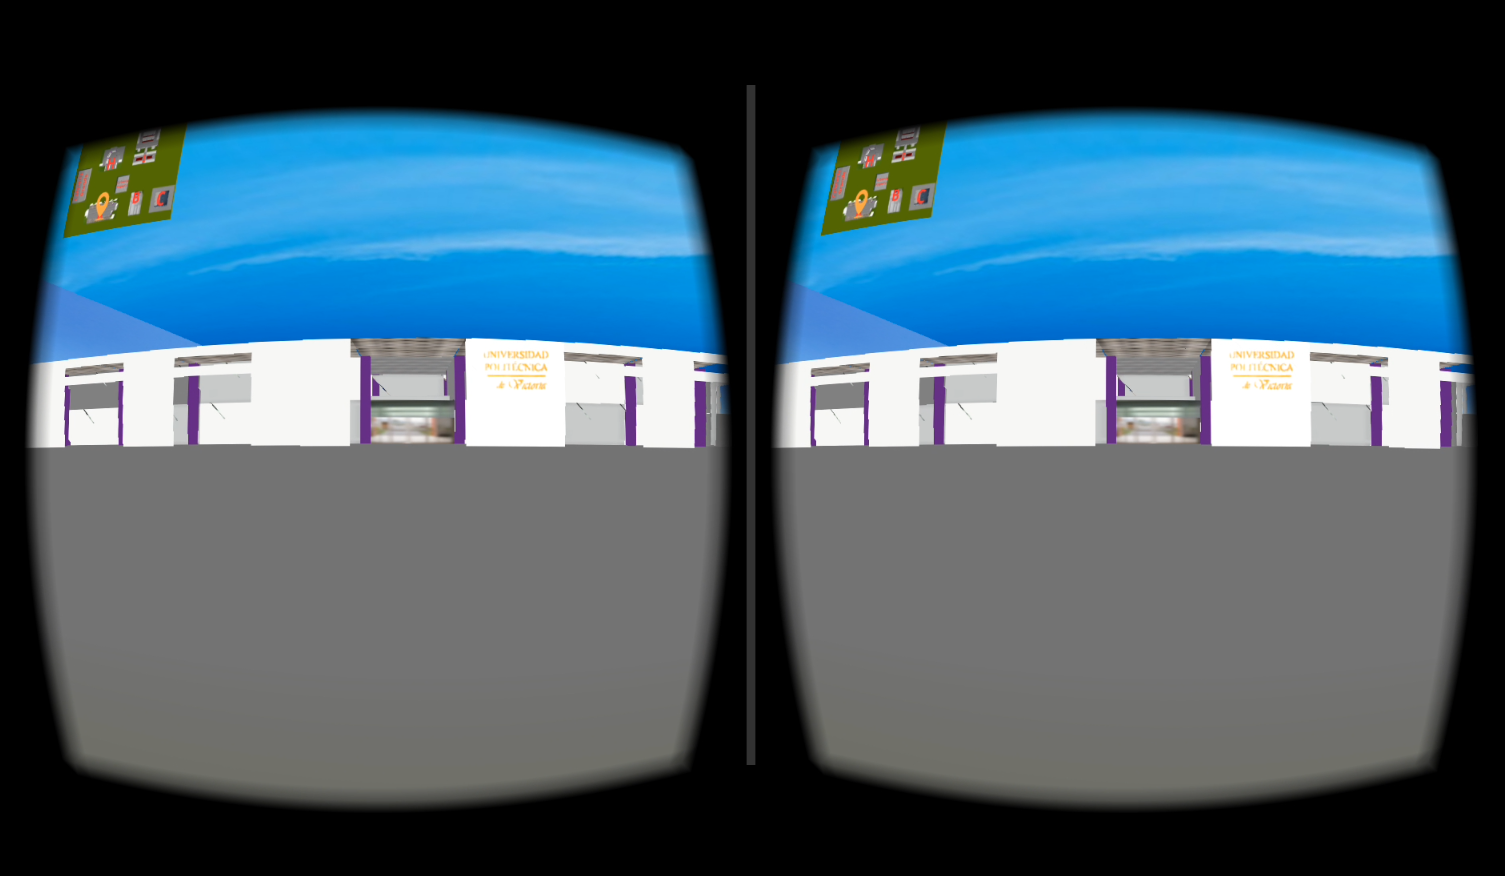
\includegraphics[width=0.85\columnwidth]{Inicio_App}\label{Inicio_App}} \\
	\vspace{0.2cm}
	\subfloat[Sincronización del minimapa.]{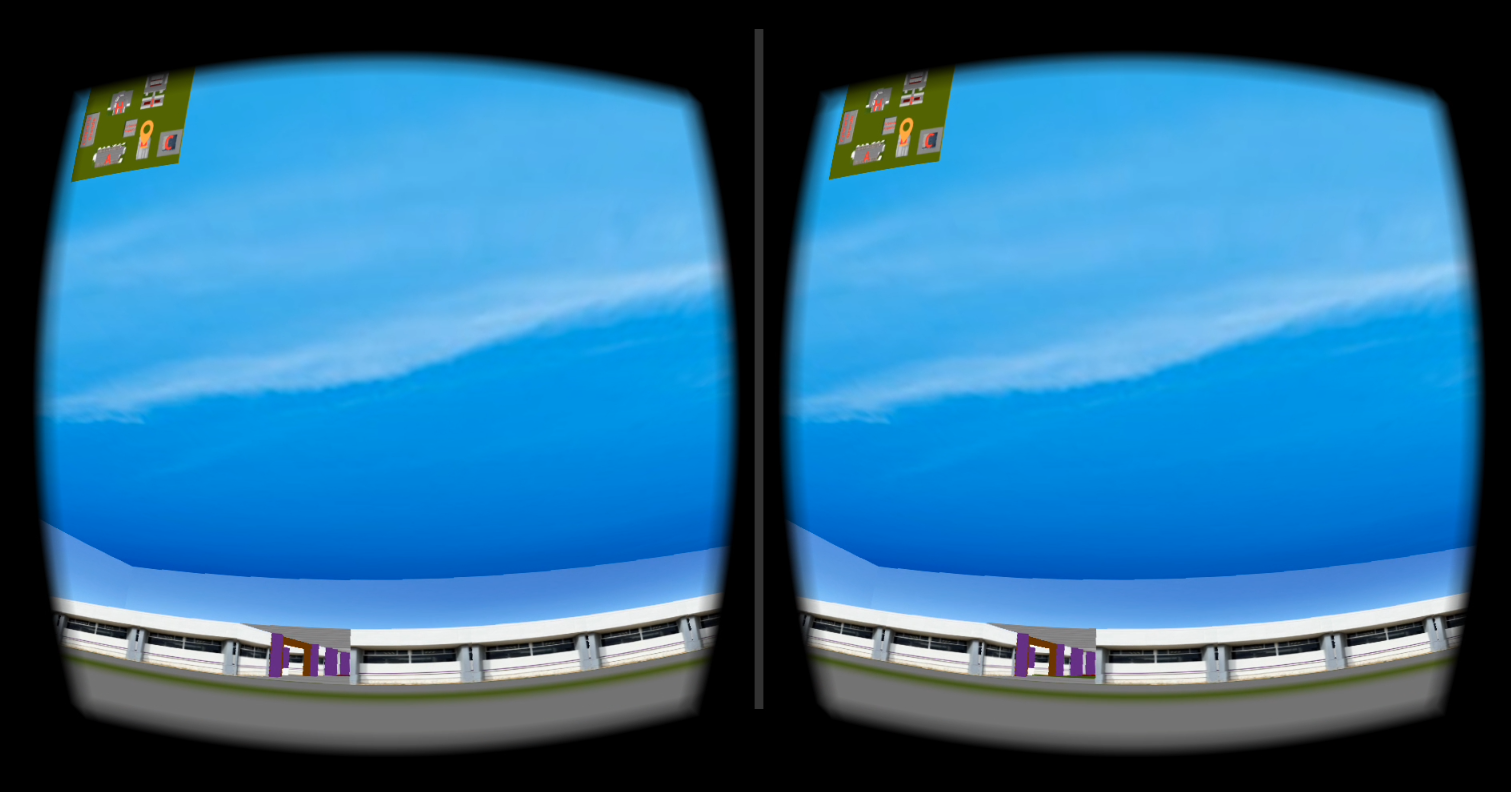
\includegraphics[width=0.85\columnwidth]{Sincronizacion_Mapa}\label{fig_mapa_sensores}}
	\caption{Estado inicial del sistema.}
	\label{fig_otros_detalles}
\end{figure}

En la Figura \ref{fig_edificio_c}(a) se observa la fachada exterior del Edificio C, destacando la correcta aplicación de texturas que dan realismo a los elementos arquitectónicos. Complementariamente, en la Figura \ref{fig_edificio_c}(b) se muestra el interior de esta misma estructura, donde se verifica que la perspectiva de la cámara permite una visualización clara de la distribución interna del edificio.

\vspace{0.3cm}

\begin{figure}[h!]
	\centering
	\subfloat[Exterior del Edificio C.]{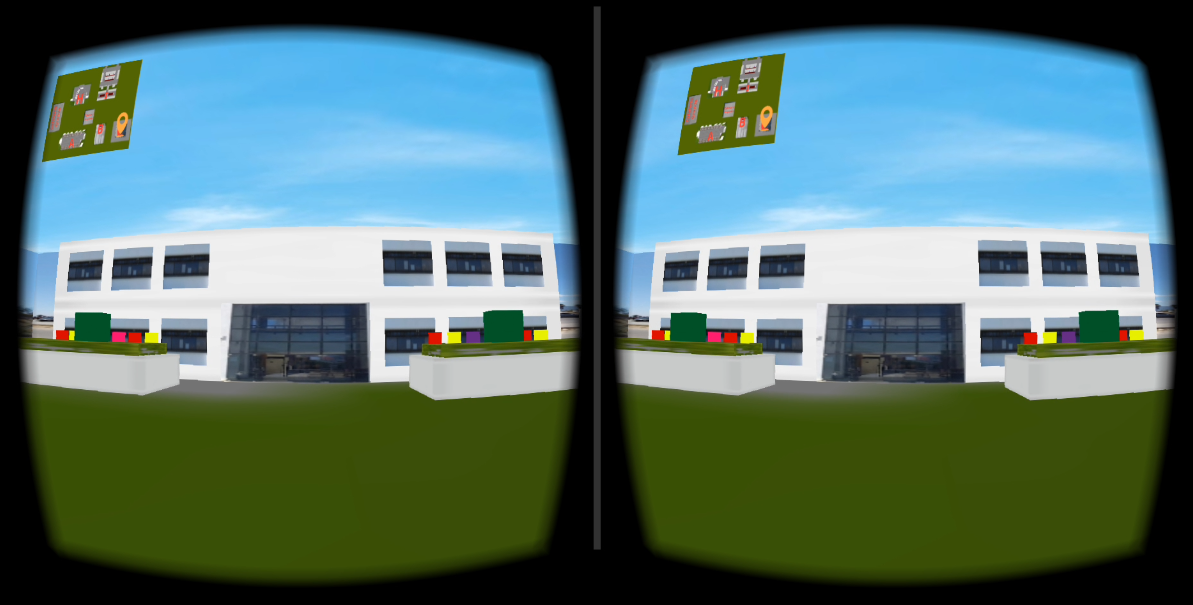
\includegraphics[width=0.83\columnwidth]{Exterior_C}\label{Fachada_C}} \\
	\vspace{0.2cm}
	\subfloat[Interior del Edificio C.]{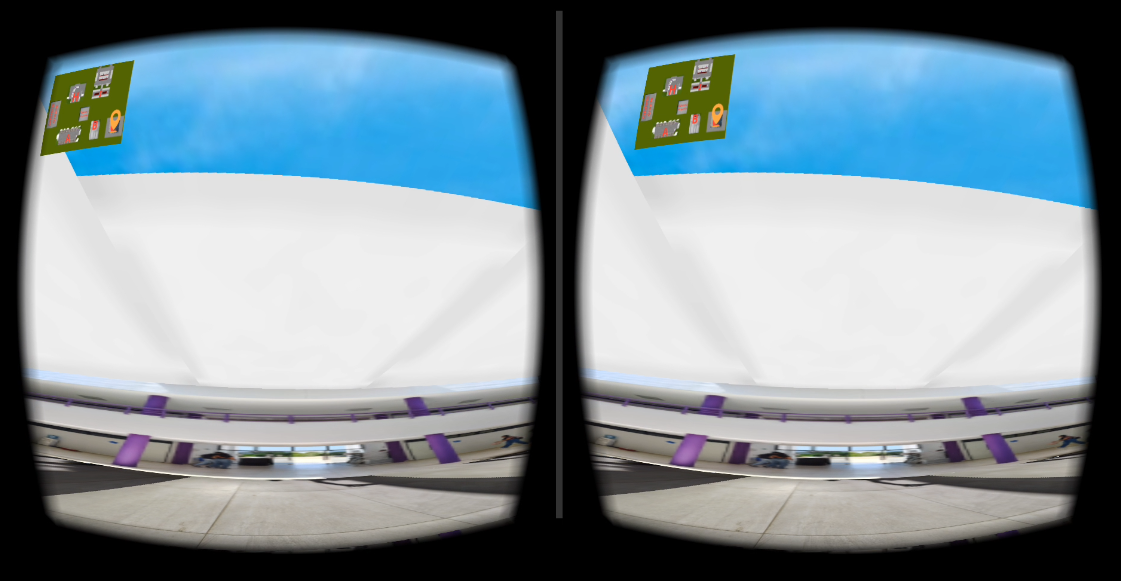
\includegraphics[width=0.83\columnwidth]{Interior_C}\label{Interior_C}}
	\caption{Visualización exterior e interior del Edificio C.}
	\label{fig_edificio_c}
\end{figure}

Respecto a la Cafetería Grande, en la Figura \ref{fig_cafeteria_grande}(a) se muestra su aspecto exterior, se muestra el letrero distintivo que permite al usuario identificar el lugar rápidamente aunque está al revés. Posteriormente, en la Figura \ref{fig_cafeteria_grande}(b) se detalla el interior del establecimiento, donde se aprecia la disposición del mobiliario como mesas y sillas.

\vspace{0.3cm}

\begin{figure}[h!]
	\centering
	\subfloat[Exterior de la Cafetería Grande.]{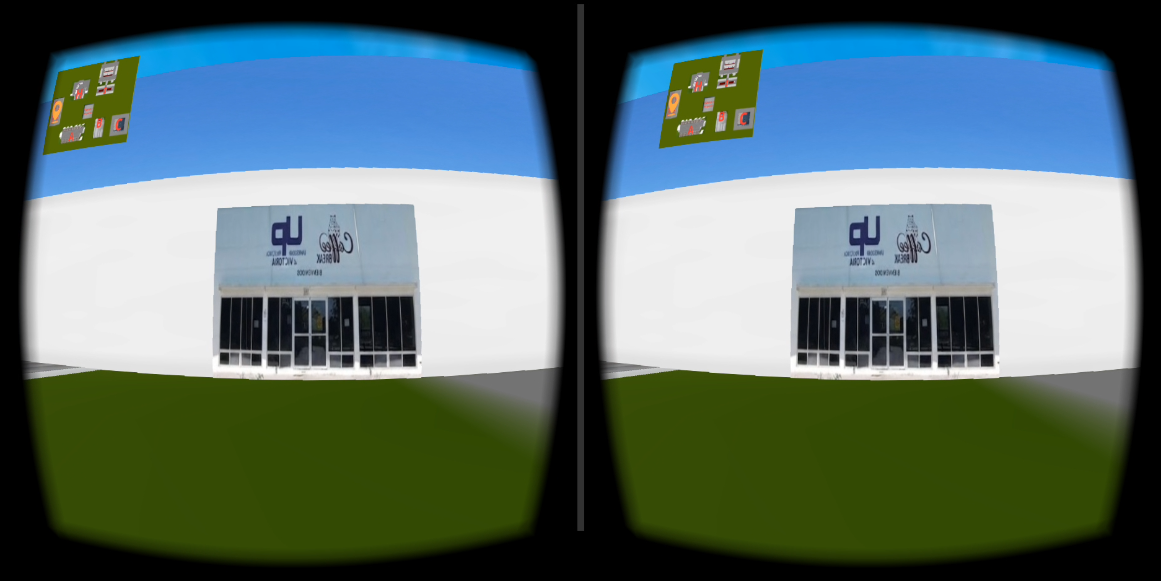
\includegraphics[width=0.93\columnwidth]{Exterior_CafeGrande}\label{Fachada_CG}} \\
	\vspace{0.2cm}
	\subfloat[Interior con mobiliario.]{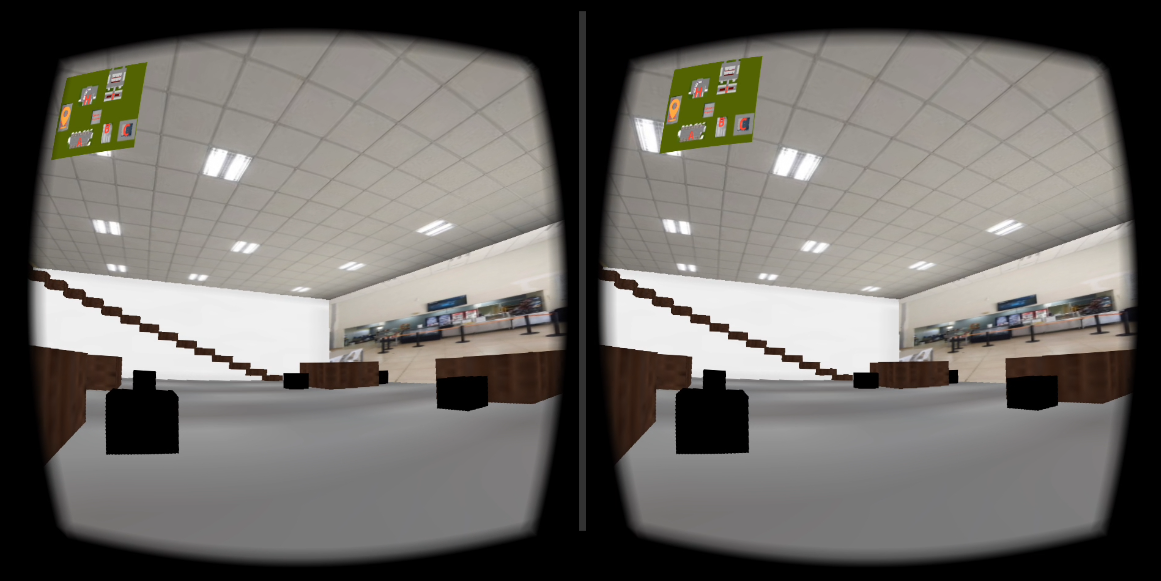
\includegraphics[width=0.93\columnwidth]{Interior_CafeGrande}\label{Interior_Cafeteria}}
	\caption{Edificio que representa la Cafetería Grande.}
	\label{fig_cafeteria_grande}
\end{figure}

Por otro lado, la Figura \ref{fig_cafeteria_pequena}(a) permite observar el exterior de la Cafetería Pequeña mientras que la Figura \ref{fig_cafeteria_pequena}(b) presenta la vista desde el interior de este pequeño edificio, demostrando que, a pesar de sus dimensiones, el sistema renderiza correctamente el espacio.

\begin{figure}[h!]
	\centering
	\subfloat[Exterior de la Cafetería Pequeña.]{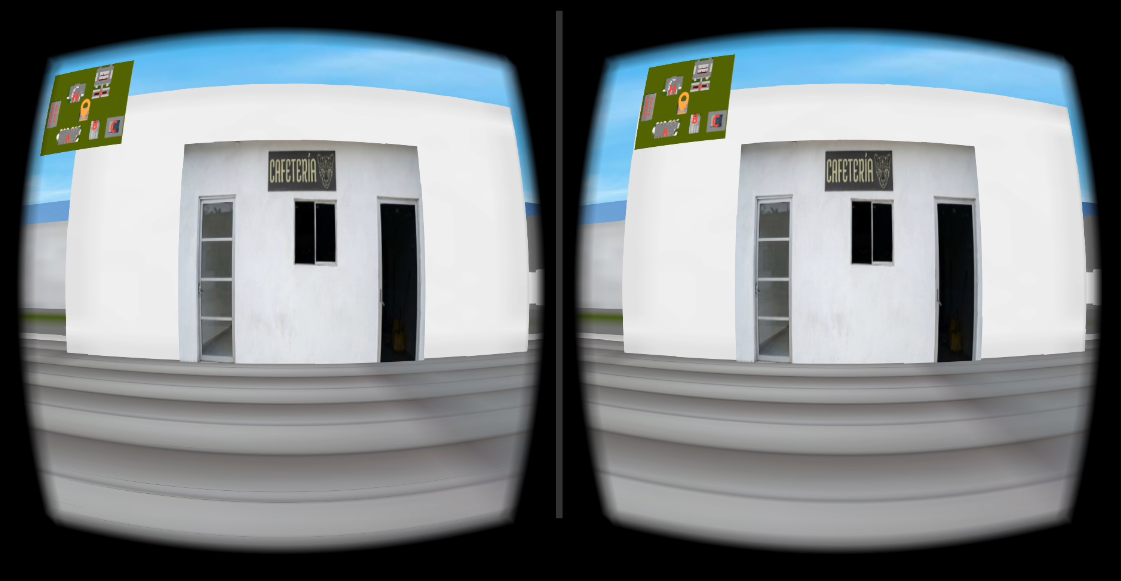
\includegraphics[width=0.93\columnwidth]{Exterior_CafePeque}\label{Fachada_CP}} \\
	\vspace{0.2cm}
	\subfloat[Vista interior de la Cafetería Pequeña.]{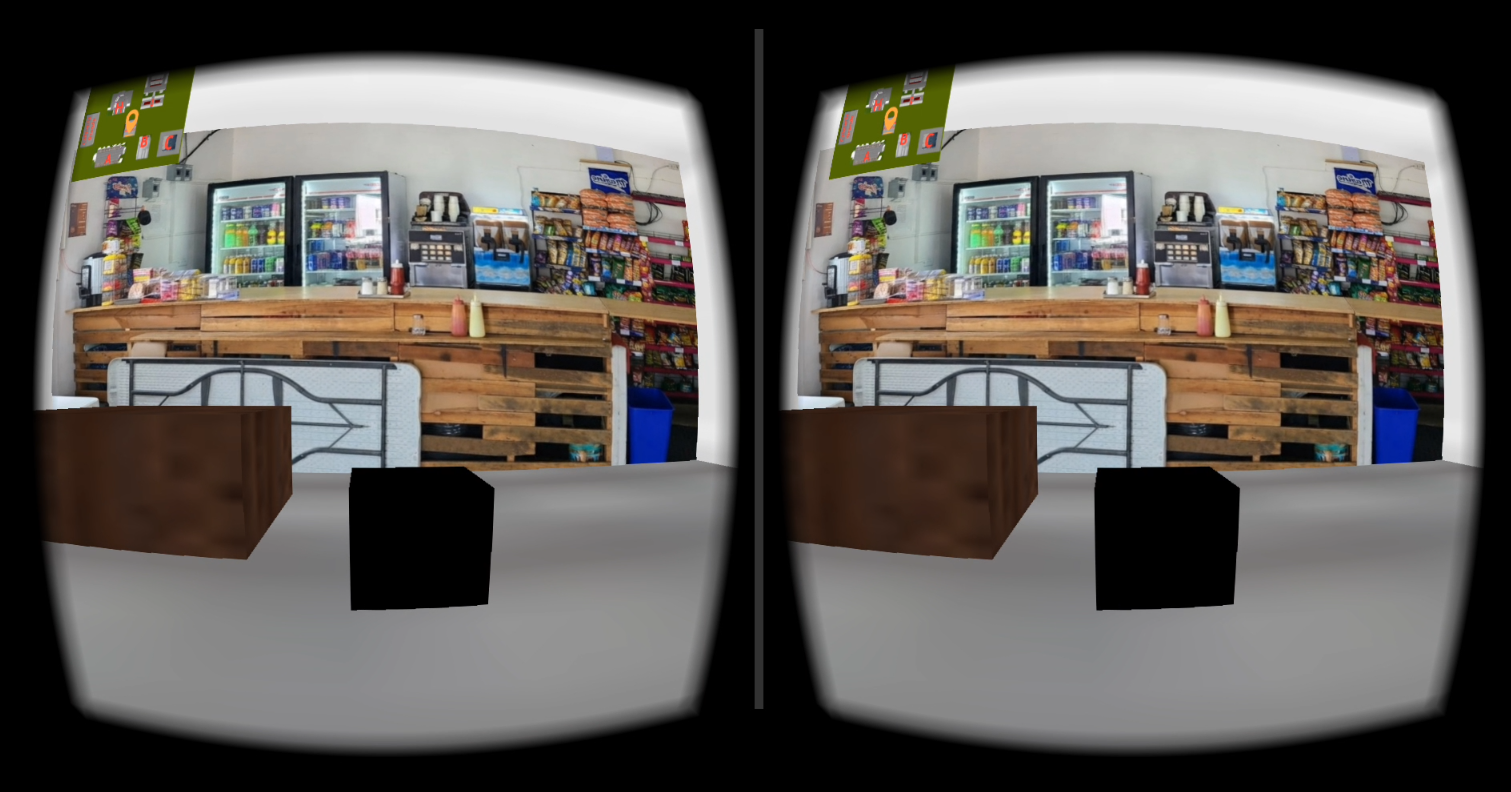
\includegraphics[width=0.93\columnwidth]{Interior_CafePeque}\label{Interior_CP}}
	\caption{Visualización de la Cafetería Pequeña.}
	\label{fig_cafeteria_pequena}
\end{figure}

Finalmente, en la Figura \ref{fig_vista_general}(a) se detalla la rotonda central y su jardinera, la cual funcionó como un elemento de referencia clave para organizar los pasillos que conectan a los edificios. Por último, la Figura \ref{fig_vista_general}(b) presenta una vista general del entorno virtual desde una perspectiva superior, permitiendo apreciar la distribución de los edificios y confirmando que su acomodo es similar al real en las instalaciones universitarias.

\vspace{0.3cm}

\begin{figure}[h!]
	\centering
	\subfloat[Detalle de la rotonda central y jardinera.]{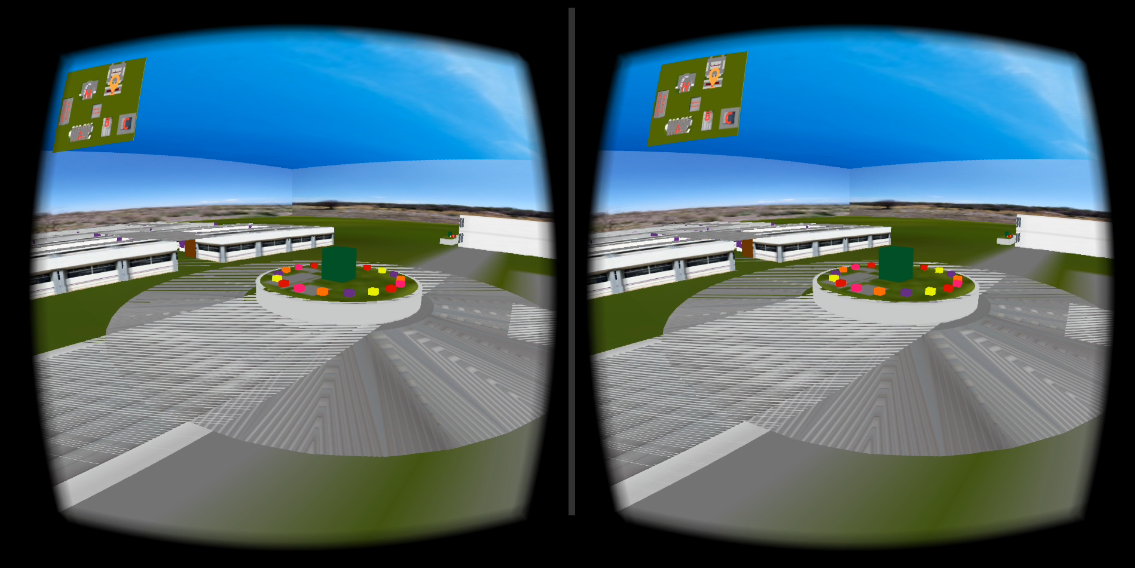
\includegraphics[width=0.97\columnwidth]{Rotonda}\label{fig_rotonda_sub}} \\
	\vspace{0.2cm}
	\subfloat[Vista general de la distribución de los edificios.]{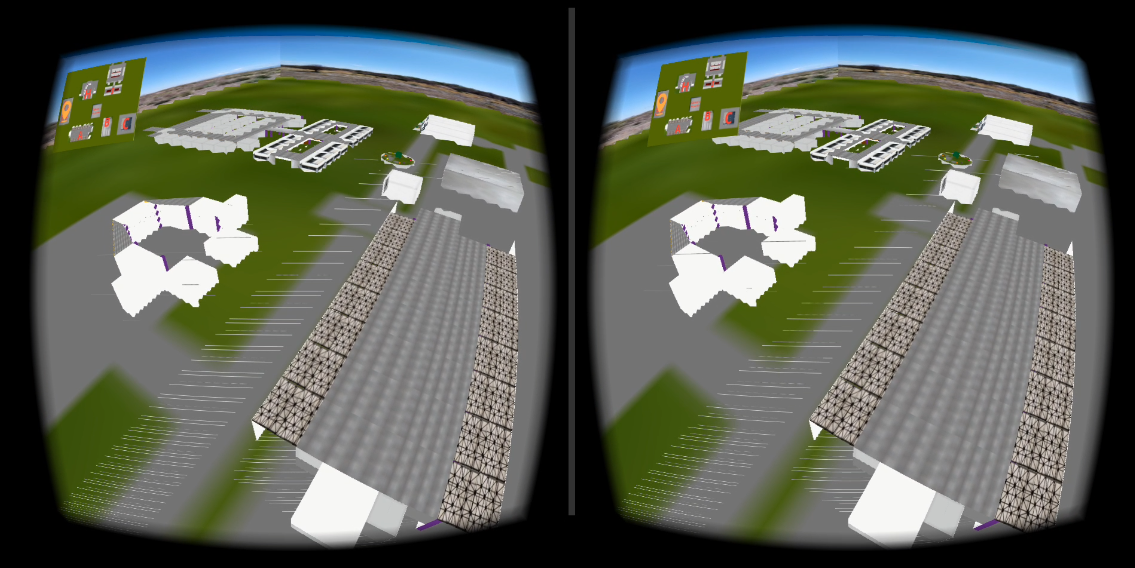
\includegraphics[width=0.97\columnwidth]{Vista_General}\label{fig_vista_general_sub}}
	\caption{Vista general de las instalaciones y rotonda central.}
	\label{fig_vista_general}
\end{figure}

\section{Conclusión}

El desarrollo de esta aplicación móvil ayudó a poner en práctica lo aprendido en clase sobre los temas de Realidad Virtual usando Android Studio, el lenguaje Java y la herramienta OpenGL para crear gráficos en 3D. 

Tomando el demo original de la universidad, ampliamos el mundo virtual para incluir los edificios C (modificado para que estuviera completo y que tenga su tragaluz y detalles por dentro), la Cafetería Grande y la Cafetería Pequeña. 

Además, acomodamos los edificios de manera similar a como están en la universidad, agregando caminos que los conectan y la rotonda con jardinera en el centro.

\vspace{0.2cm}

Durante los cambios que se realizaron al proyecto, se resolvieron problemas importantes. Uno de ellos es que se optimizaron las imágenes para que no desaparecieran cuando la cámara se aleja, y se corrigieron los sensores del celular. 

Otro problema que ocurría antes era que al mover el teléfono la vista se iba al lado contrario o se movía sola; ahora el movimiento es natural y apunta exactamente hacia donde el usuario mira. También se logró sincronizar el minimapa en tiempo real para que la persona sepa siempre en qué parte de la universidad está.

\vspace{0.2cm}

Al final, las pruebas demostraron que la aplicación funciona bien. Se puede caminar por los pasillos, entrar a los edificios, revisar los interiores y explorar las instalaciones. Con todo esto, se cumplió el objetivo principal del proyecto, logrando una herramienta digital útil e interactiva que facilita el recorrido virtual por la universidad.

\vspace{0.2cm}

Como mejoras futuras, el proyecto busca hacer que la experiencia se sienta mucho más real y completa, por lo que se puede mejorar la apariencia de las construcciones agregando texturas mucho más detalladas y variadas en las paredes, para que cada edificio tenga su propia personalidad y sea muy fácil distinguirlos a simple vista, logrando así un entorno más inmersivo y fácil de explorar para cualquier persona.

\newpage

\addcontentsline{toc}{section}{Referencias} 
\printbibliography
%\balance

\end{document}